\documentclass[a4paper]{article}

\usepackage[english]{babel}
\usepackage{amsfonts, amssymb, mathtools, amsthm, amsmath}
\usepackage{graphicx, pgfplots}
\usepackage{bm} 
\usepackage{url}
\usepackage[dvipsnames]{xcolor}
\usepackage{lastpage}
\usepackage{chngcntr}
  \counterwithin{figure}{section}
  \renewcommand{\thefigure}{\thesection.\arabic{figure}}

%loaded last
\usepackage[hidelinks]{hyperref}
\usepackage[nameinlink]{cleveref} 

\usepackage{siunitx}
  \sisetup{exponent-product = \cdot,
    output-decimal-marker = {,}}

%Giles Castelles incfig
\usepackage{import}
\usepackage{xifthen}
\usepackage{pdfpages}
\usepackage{transparent}

\newcommand{\incfig}[2][1]{%
  \def\svgwidth{#1\columnwidth}
  \import{./figures/}{#2.pdf_tex}
}

\setlength{\parindent}{0in}
\setlength{\parskip}{12pt}
\setlength{\oddsidemargin}{0in}
\setlength{\textwidth}{6.5in}
\setlength{\textheight}{8.8in}
\setlength{\topmargin}{0in}
\setlength{\headheight}{18pt}

\usepackage{fancyhdr}
\pagestyle{fancy}

\fancyhead{}
\fancyfoot{}
\fancyfoot[R]{\thepage}
\fancyhead[C]{\leftmark}

\pgfplotsset{compat=newest}

\pgfplotsset{every axis/.append style={
  axis x line=middle,    % put the x axis in the middle
  axis y line=middle,    % put the y axis in the middle
  axis line style={<->,color=black}, % arrows on the axis
}}

\usepackage{thmtools}
\usepackage{tcolorbox}
  \tcbuselibrary{skins, breakable}
  \tcbset{
    space to upper=1em,
    space to lower=1em,
  }

\theoremstyle{definition}

\newtcolorbox[auto counter]{definition}[1][]{%
  breakable,
  colframe=ForestGreen,  %frame color
  colback=ForestGreen!5, %background color
  colbacktitle=ForestGreen!25, %background color for title
  coltitle=ForestGreen!70!black,  %title color
  fonttitle=\bfseries\sffamily, %title font
  left=1em,              %space on left side in box,
  enhanced,              %more options
  frame hidden,          %hide frame
  borderline west={2pt}{0pt}{ForestGreen},  %display left line
  title=Definition \thetcbcounter: #1,
}

\newtcolorbox{greenline}{%
  breakable,
  colframe=ForestGreen,  %frame color
  colback=white,          %remove background color
  left=1em,              %space on left side in box
  enhanced,              %more options
  frame hidden,          %hide frame
  borderline west={2pt}{0pt}{ForestGreen},  %display left line
}

\newtcolorbox[auto counter, number within=section]{dis}[1][]{%
  breakable,
  colframe=NavyBlue,  %frame color
  colback=NavyBlue!5, %background color
  colbacktitle=NavyBlue!25,    %background color for title
  coltitle=NavyBlue!70!black,  %title color
  fonttitle=\bfseries\sffamily, %title font
  left=1em,            %space on left side in box,
  enhanced,            %more options
  frame hidden,        %hide frame
  borderline west={2pt}{0pt}{NavyBlue},  %display left line
  title=Discussion \thetcbcounter: #1
}

\newtcolorbox{blueline}{%
  breakable,
  colframe=NavyBlue,     %frame color
  colback=white,         %remove background
  left=1em,              %space on left side in box,
  enhanced,              %more options
  frame hidden,          %hide frame
  borderline west={2pt}{0pt}{NavyBlue},  %display left line
}

\newtcolorbox{exa}[1][]{%
  breakable,
  colframe=RawSienna,  %frame color
  colback=RawSienna!5, %background color
  colbacktitle=RawSienna!25,    %background color for title
  coltitle=RawSienna!70!black,  %title color
  fonttitle=\bfseries\sffamily, %title font
  left=1em,              %space on left side in box,
  enhanced,              %more options
  frame hidden,          %hide frame
  borderline west={2pt}{0pt}{RawSienna},  %display left line
  title=Example: #1,
}

\newtcolorbox[auto counter, number within=section]{sæt}[1][]{%
  breakable,
  colframe=RawSienna,  %frame color
  colback=RawSienna!5, %background color
  colbacktitle=RawSienna!25,    %background color for title
  coltitle=RawSienna!70!black,  %title color
  fonttitle=\bfseries\sffamily, %title font
  left=1em,              %space on left side in box,
  enhanced,              %more options
  frame hidden,          %hide frame
  borderline west={2pt}{0pt}{RawSienna},  %display left line
  title=Sætning \thetcbcounter: #1,
  before lower={\textbf{Bevis:}\par\vspace{0.5em}},
  colbacklower=RawSienna!25,
}

\newtcolorbox{redline}{%
  breakable,
  colframe=RawSienna,  %frame color
  colback=white,       %Remove background color
  left=1em,            %space on left side in box,
  enhanced,            %more options
  frame hidden,        %hide frame
  borderline west={2pt}{0pt}{RawSienna},  %display left line
}

\newtcolorbox{des}[1][]{%
  breakable,
  colframe=NavyBlue,  %frame color
  colback=NavyBlue!5, %background color
  colbacktitle=NavyBlue!25,    %background color for title
  coltitle=NavyBlue!70!black,  %title color
  fonttitle=\bfseries\sffamily, %title font
  left=1em,              %space on left side in box,
  enhanced,              %more options
  frame hidden,          %hide frame
  borderline west={2pt}{0pt}{NavyBlue},  %display left line
  title=Description of #1,
}

\makeatother
\def\@lecture{}%
\newcommand{\lecture}[3]{
  \ifthenelse{\isempty{#3}}{%
    \def\@lecture{Lecture #1}%
  }{%
    \def\@lecture{Lecture #1: #3}%
  }%
  \subsection*{\makebox[\textwidth][l]{\@lecture \hfill \normalfont\small\textsf{#2}}}
}

\makeatletter

\newcommand{\exercise}[1]{%
 \def\@exercise{#1}%
 \subsection*{Exercise #1}
}

\makeatother

%Format lim the same way in intext and in display
\let\svlim\lim\def\lim{\svlim\limits}

% horizontal rule
\newcommand\hr{
\noindent\rule[0.5ex]{\linewidth}{0.5pt}
}

\author{Noah Rahbek Bigum Hansen}



\title{Take-Home Assignment weeks 35--36}
\date{}

\begin{document}

\maketitle

\exercise{P1-1}
Determine the magnitude and coordinate direction angles of the resultant force acting at $A$.

\begin{figure} [ht]
  \centering
  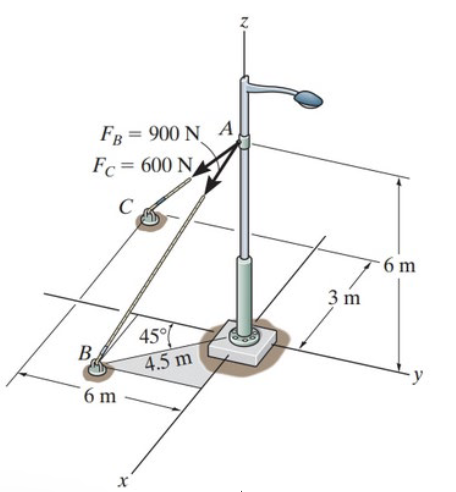
\includegraphics[width=0.5\linewidth]{../figures/P1_1}
  \label{fig:P1_1}
\end{figure}

We start by adding a coordinate system such that the point $A$ is located at the origin $O$. The resultant force here $\textbf{F}_A$ is simply the sum of the two acting forces $F_B = \qty{900}{N}$ and $F_C = \qty{600}{N}$. We must therefore express these two in terms of Cartesian coordinates. First of all we start by determining the side length of the isoceles right triangle comprised by $\textbf{r}_B$ and its components. These components can be found as:
\[ 
  \cos \ang{45} \cdot \qty{4.5}{m} = \sin \ang{45} \cdot \qty{4.5}{m} = \qty{3,18}{m}
.\]
This means that the position vector $\textbf{r}_B$ can be written as:
\[ 
\textbf{r}_B = \left( \qty{3,18}{m} \textbf{i} - \qty{3,18}{m} \textbf{j} - \qty{6}{m} \textbf{k} \right)
.\]
A unit vector along this direction can be found as:
\[ 
\textbf{u}_B = \frac{\textbf{r}_B}{\left| \textbf{r}_B \right|} = \frac{ \left( \qty{3,18}{m} \textbf{i} - \qty{3,18}{m} \textbf{j} - \qty{6}{m} \textbf{k} \right)}{\sqrt{ \left( \qty{3,18}{m}  \right)^2 + \left( \qty{3,18}{m}  \right)^2 + \left( \qty{6}{m}  \right)^2 }} = \num{0,4241}  \textbf{i} - \num{0,4241}  \textbf{j} - \num{0,8002} \textbf{k}
.\]
Now if we just multiply this by the magnitude of the force $F_B$ we get the force in the direction of $B$ in cartestian coordinates:
\[ 
\textbf{F}_B = F_B \cdot \textbf{u}_B = \qty{900}{N} \cdot \left( \num{0,4241} \textbf{i} - \num{0,4241} \textbf{j} - \num{0,8002} \textbf{k}  \right) = \qty{381,69}{N} \, \textbf{i} - \qty{381,69}{N} \, \textbf{j} - \qty{720,18}{N} \, \textbf{k}
.\]

We can also find the unit vector along $\textbf{r}_C$ as:
\[ 
\textbf{u}_C = \frac{\textbf{r}_C}{\left| \textbf{r}_C \right|} = \frac{\left( - \qty{3}{m} \, \textbf{i} - \qty{6}{m} \, \textbf{j} - \qty{6}{m}\, \textbf{k} \right)}{\sqrt{\left( \qty{3}{m}  \right)^2 + \left( \qty{6}{m}  \right)^2 + \left( \qty{6}{m}  \right)^2}} = - \num{0,333} \textbf{i} - \num{0,666} \textbf{j} - \num{0,666} \textbf{k}
.\]
Therefore we can now find $\textbf{F}_C$ as:
\[ 
\textbf{F}_C = F_C \textbf{u}_C = \qty{600}{N} \cdot \left( -\num{0,333} \textbf{i} - \num{0,666} \textbf{j} - \num{0,666}  \textbf{k} \right) = - \qty{200}{N} \, \textbf{i} - \qty{400}{N} \, \textbf{j} - \qty{400}{N} \, \textbf{k}
.\]
The resultant force $\textbf{F}_A$ can now be found as:
\[ 
  \textbf{F}_A = \textbf{F}_B + \textbf{F}_C = \qty{0,182}{kN} \, \textbf{i} - \qty{0,782}{kN} \, \textbf{j} - \qty{1,12}{kN} \, \textbf{k}
.\]
The magnitude of this can be found by the Pythagorean theorem as:
\[ 
F_A = \sqrt{\left( \qty{0,182}{kN}  \right)^2 + \left( \qty{0,782}{kN}  \right)^2 +( \qty{1,12}{kN} )^2} = \qty{1,38}{kN} 
.\]
Now we can find the angles with each of the three axes as:
\begin{align*}
  \alpha &= \cos^{-1} \left( \frac{F_{Ax}}{F_A} \right) = \cos^{-1} \num{0,132} = \ang{82,4} \\
  \beta &= \cos^{-1} \left( \frac{F_{Ay}}{F_A} \right) = \cos^{-1} \num{-0,567} = \ang{124,5}  \\
  \gamma &= \cos^{-1} \left( \frac{F_{Az}}{F_A} \right) = \cos^{-1} \num{-0,813} = \ang{144,4} 
.\end{align*}
Therefore the resultant force $\textbf{F}_A$ is of magnitude \qty{1,38}{kN} and makes angles of \ang{82,4}, \ang{124,5}, and \ang{144,4} with the positive $x$-, $y$-, and $z$-axes respectively. 


\end{document}
